\subsection{Endpoint fanout}

The Endpoint fanout contains configurable amount of Endpoint
modules connected together with the Wishbone Crossbar.\\

Base Wishbone addresses of Endpoints:\\

\begin{tabular}{|l|l|}
  \hline
  module name & base address\\
  \hline \hline
  \emph{Endpoint 0} & 0x30000\\
  \emph{Endpoint 1} & 0x30400\\
  \emph{Endpoint 2} & 0x30800\\
  \emph{Endpoint 3} & 0x30c00\\
  \emph{Endpoint 4} & 0x31000\\
                ... & ...\\
  \emph{Endpoint n} & 0x30000 + n*0x400\\
  \hline
\end{tabular}\\

\noindent {\bf Description:}

Endpoint module implements Gigabit Ethernet MAC functionality and PCS for
Gigabit optical link. It sends and receives Ethernet frames from a physical link
and is able to generate precise Tx and Rx timestamps. It also has VLAN and Flow
Control (receiving Pause frames) support. 

Additionally it is able to inject frames required by the Topology Resolution
Unit (sec. \ref{sec:tru}) for hardware supported RSTP and generates events
counted by Per-port Statistics module (sec. \ref{sec:pstats}).

Endpoint contains also a programmable packet filter, which can classify
incoming Ethernet frames into 8 different classes.\\

\noindent{\bf Wishbone interface:} section \ref{subsec:wbgen:ep}.

\subsubsection{Programmable packet filter}
The description of the packet filter inside the
Endpoint module is taken from \emph{dev/ep\_pfilter.c} file stored in
White Rabbit PTP Core Software repository.\\

The classifier processes the incoming frame, and assigns it to one of 8 classes
(an 8-bit word, where each bit corresponds to a particular class) or eventually
drops it. Hardware implementation of the unit is a simple VLIW processor with 32
single-bit registers (0 - 31). The registers are organized as follows:
\begin{itemize}
  \item 0: don't touch (always 0)
  \item 1 - 22: general purpose registers
  \item 23: drop frame flag: if 1 at the end of the frame processing, the frame will be dropped.
  \item 24..31: packet class (class 0 = reg 24, class 7 = reg 31).
\end{itemize}

Program memory has 64 36-bit words. Packet filtering program is restarted every
time a new frame comes.
There are 5 possible instructions:

\begin{enumerate}
  \item \emph{CMP offset, value, mask, oper, Rd}:\\
    Rd = Rd oper ((((uint16\_t *)frame) [offset] \& mask) == value)
    
    \underline{Examples:}
    \begin{itemize}
      \item \emph{CMP 3, 0xcafe, 0xffff, MOV, Rd}\\
            will compare the 3rd word of the frame (bytes 6, 7) against 0xcafe
            and if the words are equal, 1 will be written to Rd register.
      \item \emph{CMP 4, 0xbabe, 0xffff, AND, Rd}\\
            will do the same with the 4th word and write to Rd its previous
            value ANDed with the result of the comparison. Effectively, Rd now
            will be 1 only if bytes [6..9] of the payload contain word
            0xcafebabe.
    
            Note that the mask value is nibble-granular. That means you can
            choose a particular set of nibbles within a word to be compared, but
            not an arbitrary set of bits (e.g. 0xf00f, 0xff00 and 0xf0f0 masks
            are ok, but 0x8001 is wrong.
    \end{itemize}

  \item \emph{BTST offset, bit\_number, oper, Rd}:\\
    Rd = Rd oper (((uint16\_t *)frame) [offset] \& (1$\ll$bit\_number) ? 1 : 0)

    \underline{Examples:}
    \begin{itemize}
      \item \emph{BTST 3, 10, MOV, 11}\\
            will write 1 to reg 11 if the 10th bit in the 3rd word of the frame 
            is set (and 0 if it's clear)
    \end{itemize}

  \item Logic opearations:
    \begin{itemize}
      \item \emph{LOGIC2 Rd, Ra, OPER Rb} - 2 argument logic (Rd = Ra OPER Rb). If the
            operation is MOV or NOT, Ra is taken as the source register.
      \item \emph{LOGIC3 Rd, Ra, OPER Rb, OPER2, Rc} - 3 argument logic Rd = (Ra
            OPER Rb) OPER2 Rc.
    \end{itemize}

  \item Miscellaneous:
    \begin{itemize}
      \item \emph{FIN} instruction terminates the program.
      \item \emph{NOP} executes a dummy instruction (LOGIC2 0, 0, AND, 0)
    \end{itemize}
\end{enumerate}

IMPORTANT:
\begin{itemize}
  \item the program counter is advanced each time a 16-bit words of the frame arrives.
  \item the CPU doesn't have any interlocks to simplify the HW, so you can't
    compare the 10th word when PC = 2. Max comparison offset is always equal to
    the address of the instruction.
  \item Code may contain up to 64 operations, but it must classify shorter frames faster than in
  32 instructions (there's no flow throttling)
\end{itemize}

\subsubsection{Injection engine}
The frame injection engine has to be programmed first with frames' templates
and after that sending (injecting) each template can be triggered from the TRU
module.

Storing frame templates is done through the \emph{VCR1} Wishbone register. Each
word written to this register is a concatenation of the offset value and the data
word (check section \ref{subsec:wbgen:ep}). Since the same block RAM is shared
by the Injection engine and VLAN unit, templates have to be stored starting with
the offset {\bf 512}. This buffer can store up to 8 templates each not longer
than 128 bytes.

Storing a frame's template requires splitting such frame into 2-byte words and
performing a set of writes into the \emph{VCR1} register (each time the offset
value has to be incremented). The format of data word is presented in figure
\ref{fig:ep:inject_data}:
\begin{figure}[ht]
  \begin{center}
    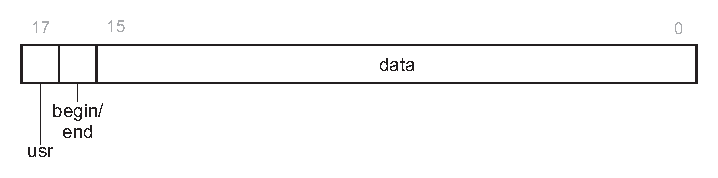
\includegraphics[width=.8\textwidth]{switch/ep_inject.ps}
    \caption{Format of data word for programming the injection engine}
    \label{fig:ep:inject_data}
  \end{center}
\end{figure}

\begin{tabular}{l p{13cm}}
  \emph{data} & 2-byte chunk of the template\\
  \emph{begin/end} & if set to 1, the written word is first or last word of
    template's data\\
  \emph{usr} & if set to 1, this data word will be replaced by the value
    provided by the TRU module\\
\end{tabular}
